\documentclass[11pt,a4paper]{article}

\usepackage{fontspec}
\usepackage{amsmath,amssymb}
\usepackage[margin=2.5cm,headheight=14pt]{geometry}
\usepackage{microtype}
\usepackage{xcolor}
\usepackage{graphicx}
\usepackage{booktabs}
\usepackage{tabularx}
\usepackage{longtable}
\usepackage{array}
\usepackage{enumitem}
\usepackage{fancyhdr}
\usepackage{caption}
\usepackage{float}
\usepackage{algorithm}
\usepackage{algpseudocode}
\usepackage{tikz}
\usetikzlibrary{arrows.meta,positioning,fit,calc}
\usepackage{pgfplots}
\pgfplotsset{compat=1.18}
\usepackage[colorlinks=true,linkcolor=blue!60!black,urlcolor=blue!60!black,citecolor=blue!60!black]{hyperref}

\setlength{\parindent}{0pt}
\setlength{\parskip}{5pt}
\setlist{itemsep=2pt,topsep=3pt}
\renewcommand{\arraystretch}{1.18}

\usepackage{xurl}
\DeclareUrlCommand\code{\urlstyle{tt}}
\emergencystretch=2em
\newcolumntype{L}{>{\raggedright\arraybackslash}X}

% Screenshot placeholder: replace the \fbox{...} with \includegraphics[width=\linewidth]{file.png}
\newcommand{\screenshot}[3]{%
\begin{figure}[htbp]\centering
\fbox{\parbox[c][5.2cm][c]{0.92\linewidth}{\centering\small
\textbf{[SCREENSHOT PLACEHOLDER]}\\[6pt]#2}}
\caption{#1}\label{#3}
\end{figure}}

\pagestyle{fancy}
\fancyhf{}
\fancyhead[L]{\small ACO TSP Solver -- Technical Documentation}
\fancyhead[R]{\small\thepage}
\renewcommand{\headrulewidth}{0.4pt}
\fancypagestyle{plain}{\fancyhf{}\fancyfoot[C]{\thepage}\renewcommand{\headrulewidth}{0pt}}

\begin{document}

\thispagestyle{plain}
\begin{center}
\vspace*{1.2cm}
{\LARGE\bfseries ACO TSP Solver}\\[10pt]
{\large Ant Colony Optimization for the Travelling Salesman Problem}\\[2pt]
{\large Ant System on natID Dense Matrices with Real-Time Visualization}\\[16pt]
{\large Armin Memišević} \quad (index 20016)\\[4pt]
Faculty of Electrical Engineering (ETF), University of Sarajevo\\
Course: Numerical Optimization --- Prof. Dr. Izudin Džafić\\[10pt]
{\large Academic Year 2025/26}
\end{center}

\vspace{0.6cm}
\begin{center}\textbf{Abstract}\end{center}
\begin{quote}\small
This document describes \textbf{ACO TSP Solver} (build target \code{tspaco}, version 1.1), a desktop
C++ application that solves the \textbf{Travelling Salesman Problem (TSP)} with the
\textbf{Ant System}, the original \textbf{Ant Colony Optimization (ACO)} algorithm of Dorigo and Stützle.
Each problem instance consists of 15--25 cities drawn at random from a set of 99 real towns in Bosnia and
Herzegovina with true geographic coordinates. The application builds the $n\times n$ distance matrix and the $n\times n$ pheromone matrix
as \code{dense::DblMatrix} objects from the natID matrix library, and lets a colony of artificial ants
construct tours by roulette-wheel selection driven by pheromone intensity ($\alpha$) and inverse
distance ($\beta$). After every iteration the trail is evaporated and reinforced in proportion to
$Q/L_k$, using whole-matrix library operators for the evaporation and deposit-application steps. Every
tour is checked for feasibility (a genuine permutation of all cities) before it is costed or allowed to
deposit pheromone. The search runs on a background thread while an interactive GUI, built on the
\code{natGUI} framework and adapted from the professor's \code{B_S03_Maps} example, renders the cities,
the best tour, the pheromone trail as edge thickness, a live convergence chart with a
nearest-neighbour baseline, and a statistics sidebar. The application additionally supports new random
instances on demand, seeded reproducibility, CSV export of the run and of the full problem instance,
side-by-side comparison of the last two completed runs, and an English/Bosnian user interface.
\end{quote}

\tableofcontents
\newpage

%=====================================================================
\section{Introduction}
%=====================================================================

\subsection{What This Project Is}
ACO TSP Solver is the term project for the Numerical Optimization course. It implements a complete
Ant Colony Optimization solver for the symmetric Travelling Salesman Problem: given $n$ cities, find the
shortest closed tour that visits each city exactly once and returns to its starting point.

The project deliberately implements the \emph{basic} Ant System rather than one of its later
refinements (Ant Colony System, MAX--MIN Ant System) and adds no local search. This keeps every number
the application reports traceable to a single, textbook update rule: whatever tour the colony finds, it
found through probabilistic construction and pheromone feedback alone.

\subsection{Why a Metaheuristic Instead of Exact Search}
The TSP is NP-hard. For $n$ cities the number of distinct undirected tours is $(n-1)!/2$, which is
$4.4\times10^{10}$ for the smallest instance the application generates ($n=15$) and $3.1\times10^{23}$ for
the largest ($n=25$). Exhaustive enumeration is out of the question. The best general exact method, the
Held--Karp dynamic program, runs in $O(n^2 2^n)$ time and $O(n\,2^n)$ memory; at $n=25$ that is on the
order of $2\times10^{10}$ operations over a table of roughly $8\times10^{8}$ entries (several gigabytes).

Ant Colony Optimization trades the guarantee of optimality for a controllable amount of computation:
$m$ ants, each building one tour in $O(n^2)$, per iteration. Section~\ref{sec:numcheck} shows that, with the
default parameters, on generated instances small enough to solve exactly ($n\le20$) the colony's best tour
was on average within 0.7\% of the true optimum.

\subsection{Project Goals}
\begin{itemize}
  \item Formulate the TSP as a combinatorial minimization problem over permutations of $n$ cities.
  \item Store the $n\times n$ distance matrix $D$ and the $n\times n$ pheromone matrix $\tau$ as natID
        dense matrices, and perform evaporation and the deposit update directly on them.
  \item Implement probabilistic tour construction by roulette-wheel selection weighted by
        $\tau_{ij}^{\alpha}\,\eta_{ij}^{\beta}$, with all parameters constant during a run.
  \item Implement the Ant System global pheromone update: evaporation followed by a deposit of $Q/L_k$
        from every ant.
  \item Run the iteration loop on a background thread, adapted from the \code{B_S03_Maps} thread
        architecture, so the interface stays responsive.
  \item Visualize the search live: cities, current best tour, pheromone strength as edge thickness, a
        convergence curve (cost vs.\ iteration), and a sidebar with iteration count, best cost and
        runtime.
\end{itemize}

\subsection{Relationship to the Original Proposal}
The project proposal (\emph{Ant Colony Optimization for the Traveling Salesman Problem}) named Dorigo \&
Stützle's \emph{Ant Colony Optimization} (MIT Press, 2004) as the theoretical source and the professor's
natID example \code{B_S03_Maps} as the starting point. The delivered implementation follows both. The
table below lists every item of the proposal against what was delivered.

\begin{longtable}{@{}p{3.6cm}p{5.2cm}p{6.2cm}@{}}
\toprule
\textbf{Item} & \textbf{Proposal} & \textbf{Delivered (+ additions)} \\
\midrule
\endhead
Problem instance & 15--25 randomly generated cities & 15--25 cities \emph{randomly selected} from 99 real Bosnian towns
  (\code{res/maps/Bosnia.xml}), with real latitude/longitude. + \emph{New cities} action draws a fresh instance at any time. \\
Distance matrix & $N\times N$ natID dense matrix & \texttt{dense::DblMatrix \_dist}, in kilometres. \\
Pheromone matrix & $N\times N$ natID dense matrix & \texttt{dense::DblMatrix \_pheromone}, plus a separate \texttt{dense::DblMatrix \_deltaPheromone} for $\Delta\tau$. \\
Tour construction & Roulette-wheel selection with $\alpha$, $\beta$ & Implemented (\code{Model::constructTour}). + Every tour validated as a Hamiltonian cycle (\code{isHamiltonianTour}). \\
Pheromone update & Evaporation + deposit $\propto 1/L$ & Implemented as $\tau\leftarrow(1-\rho)\tau$, $\Delta\tau=\sum_k Q/L_k$, $\tau\leftarrow\tau+\Delta\tau$. \\
Parameters & $\alpha,\beta,\rho$, ants, iterations constant during a run & Implemented: read once when Start is pressed. + Editable between runs, range-clamped, persisted across restarts. \\
Background thread & Adapted from \code{B_S03_Maps} & Implemented (\code{std::thread} in \code{Model::findPath}). \\
Convergence curve & Best cost vs.\ iteration, live & Implemented. + Per-iteration best curve and a repetitive nearest-neighbour reference line. \\
Map canvas & Cities, best tour, pheromone as edge thickness & Implemented. + Two pheromone display modes (All edges / Threshold) and selectable colours. \\
Sidebar & Iteration, best cost, runtime & Implemented. + Iteration of best, nearest-neighbour baseline, signed improvement, cities, ants, seed, status. \\
Controls & Start / Stop / Reset & Implemented (menu and toolbar). \\
\multicolumn{3}{@{}l}{\textit{Not in the proposal, additionally delivered:}}\\
Reproducibility & -- & Seed field (0 = random); seed and city-draw index recorded in exports. \\
Analysis & -- & CSV export (convergence series + full problem instance); comparison of the last two completed runs. \\
Usability & -- & English/Bosnian UI, Settings dialog, in-app Help, light/dark colour defaults, sounds. \\
Distribution & -- & GitHub Actions workflow building Windows, macOS (Apple Silicon, Intel) and Linux packages. \\
\bottomrule
\end{longtable}

The only substantive deviation from the literal wording of the proposal is the instance itself:
instead of synthetic random points, the cities are a random subset of real towns, so the distance
matrix reflects actual geography. Tour lengths are therefore reported in kilometres.

\subsection{Starting Point: \texttt{B\_S03\_Maps}}
From the professor's example the project keeps the application skeleton (\code{Application},
\code{MainWindow}, \code{MenuBar}, \code{ToolBar}), the \code{Town}/\code{Primitive} drawing classes, the
XML map loading in \code{ViewMap}, the canvas animation loop, and the background thread with its
completion callback. What was removed or replaced:
\begin{itemize}
  \item The \code{Graph} adjacency structure and the \code{<Roads>} network are gone. ACO needs a complete
        graph; every pair of selected cities is directly connected by its air distance. With a random
        subset of towns, the original road network would also have survived only as a few disconnected
        edges.
  \item The breadth-/depth-first search in the model was replaced by the ACO engine
        (\code{Model::runACO}), and the source/goal town pair by a single \emph{start marker} (a TSP tour
        has no separate goal).
  \item The convergence chart, statistics sidebar, compare and help dialogs, CSV export and all ACO
        parameter controls are new.
\end{itemize}

%=====================================================================
\section{Logic: Mathematical Model}
%=====================================================================

\subsection{The TSP as an Optimization Problem}
Let $V=\{1,\dots,n\}$ be the selected cities and $d_{ij}=d_{ji}\ge 0$ the distance between cities $i$ and
$j$. A tour is a cyclic permutation $\pi=(\pi_1,\dots,\pi_n)$ of $V$. The problem is
\begin{equation}
\min_{\pi\in S_n}\; f(\pi)=\sum_{i=1}^{n-1} d_{\pi_i\pi_{i+1}} + d_{\pi_n\pi_1}
\qquad\text{s.t. each city appears in }\pi\text{ exactly once.}
\label{eq:tsp}
\end{equation}
The decision space is discrete and the feasible set is exactly the set of Hamiltonian cycles of the
complete graph on $V$. ACO is the solver for~\eqref{eq:tsp}; the constraint is enforced both
structurally (an ant can only move to an unvisited city) and explicitly, by the feasibility check of
Section~\ref{sec:feas}.

\subsection{Problem Instance and Distance Model}
\code{res/maps/Bosnia.xml} contains 99 towns (latitudes 42.71--45.18$^\circ$N, longitudes
15.80--19.34$^\circ$E). On every load, \code{Model::loadTowns()} shuffles the full list with a seeded
Mersenne Twister, draws the instance size uniformly from $\{15,\dots,25\}$, and keeps that many towns.

Distances use a local equirectangular approximation with fixed kilometres-per-degree factors taken from
the map file (\code{ratioLat="111"}, \code{ratioLong="80"}; the latter is $111.3\cos 44.2^\circ\approx 79.8$
at the country's mean latitude):
\begin{equation}
d_{ij}=\sqrt{\bigl(80\,(\lambda_i-\lambda_j)\bigr)^2+\bigl(111\,(\varphi_i-\varphi_j)\bigr)^2}\ \ \text{km},
\label{eq:dist}
\end{equation}
where $\lambda$ is longitude and $\varphi$ latitude in degrees. In code the computation goes through the
normalized $[0,1]$ display coordinates of each town, multiplied by the ratios scaled by the bounding-box
span (\texttt{setDistanceRatios(ratioLat*dy, ratioLong*dx)}); the bounding-box offsets and display margins
cancel, so the result is~\eqref{eq:dist} up to single-precision rounding. Section~\ref{sec:numcheck} quantifies the approximation
error against great-circle distance.

\subsection{Distance Matrix}
\code{Model::buildDistanceMatrix()} allocates \code{_dist} with \texttt{reserve(n, n, nullptr, true)},
clears it with \code{zeros()} (the storage may be reused from a larger previous instance), and fills the
strict upper triangle, mirroring each value into the lower triangle. The diagonal stays zero.

The matrix is built once in \code{loadTowns()}, immediately after the towns are placed, so that the
nearest-neighbour baseline (Section~\ref{sec:nn}) is available before any run starts. \code{runACO()}
rebuilds it once more at the start of every run on the worker thread; this costs $O(n^2)$ and guarantees
the solver never operates on a stale matrix.

\subsection{Pheromone Matrix and Initialization}
\code{Model::initPheromone()} allocates \code{_pheromone} and \code{_deltaPheromone} with the same
dimensions, zeros both, and sets every \emph{off-diagonal} entry of $\tau$ to $\tau_0$:
\begin{equation}
\tau_{ij}^{(0)}=\begin{cases}\tau_0, & i\neq j\\ 0, & i=j\end{cases}\qquad \tau_0=1.0 .
\end{equation}
The diagonal is left at zero on purpose. A self-loop is never a legal move, so $\tau_{ii}$ is never read
during construction and never written by a deposit. Seeding it with $\tau_0$ would not change the search,
but it would decay under evaporation and distort the column sums used by the pheromone norm
(Section~\ref{sec:conv}).

\subsection{Probabilistic Tour Construction}
Each iteration launches $m$ ants. Following the Ant System, each ant starts at a city drawn uniformly at
random from $V$ (\code{startPick(rng)}); starting all ants at one fixed city would not change which tours
are reachable, but it would correlate their first decisions. An ant at city $i$ with the set
$\mathcal N_i^k$ of still-unvisited cities moves to $j\in\mathcal N_i^k$ with probability
\begin{equation}
p_{ij}^k=\frac{\tau_{ij}^{\alpha}\,\eta_{ij}^{\beta}}{\sum_{l\in\mathcal N_i^k}\tau_{il}^{\alpha}\,\eta_{il}^{\beta}},
\qquad
\eta_{ij}=\begin{cases}1/d_{ij}, & d_{ij}>10^{-6}\\ 10^{6}, & \text{otherwise.}\end{cases}
\label{eq:prob}
\end{equation}
The guard on $\eta$ prevents a division by zero for coincident cities. Selection is an explicit roulette
wheel in \code{constructTour()}: the unnormalized weights $w_l=\tau_{il}^{\alpha}\eta_{il}^{\beta}$ are
accumulated into $\Sigma$, a number $r\sim U[0,\Sigma)$ is drawn, and the first candidate whose running
sum reaches $r$ is chosen. If $\Sigma\le 0$ (which can only happen if every candidate's weight underflows to zero), the
next city is chosen uniformly among the candidates instead. $\tau_{ij}$ and $d_{ij}$ are read directly from
the two dense matrices through their manipulators.

\subsection{Feasibility Check}\label{sec:feas}
\code{Model::isHamiltonianTour()} accepts a tour only if it has exactly $n$ entries, every id is in
$1..n$, and no id repeats. It is applied twice:
\begin{enumerate}
  \item in \code{runACO()}, \emph{before} a tour is costed, compared with the incumbent, or stored for
        the deposit step; a rejected ant leaves an empty slot and contributes to nothing;
  \item in \code{depositPheromone()}, as a second line of defence (which also skips the empty slots).
\end{enumerate}
The construction procedure cannot currently produce an infeasible tour. The check exists because the
failure would be silent and severe: a short, infeasible tour is \emph{cheaper} than any real one, so it
would become the reported best, be drawn on the map, and bias every subsequent ant through its deposit.

The tour length is $L_k=f(\pi^k)$ from~\eqref{eq:tsp}, including the closing edge back to the first city
(\code{Model::tourLength}).

\subsection{Global Pheromone Update (Ant System)}
After all ants of an iteration have finished, the trail is updated in three named steps that map
one-to-one onto the Ant System rule:
\begin{align}
\tau &\leftarrow (1-\rho)\,\tau \label{eq:evap}\\
\Delta\tau_{ij} &\leftarrow \sum_{k=1}^{m}\Delta\tau_{ij}^k,\qquad
\Delta\tau_{ij}^k=\begin{cases}Q/L_k,&(i,j)\in T^k\\0,&\text{otherwise}\end{cases} \label{eq:dep}\\
\tau &\leftarrow \tau+\Delta\tau \label{eq:apply}
\end{align}
\begin{center}
\begin{tabularx}{\linewidth}{@{}c p{5.2cm} L@{}}
\toprule
\textbf{Step} & \textbf{Method} & \textbf{Operation on the natID matrix} \\
\midrule
\eqref{eq:evap} & \code{evaporatePheromone()} & \texttt{\_pheromone *= 1 - rho} \\
\eqref{eq:dep} & \code{beginPheromoneDeposit()}, \code{depositPheromone()} & \code{_deltaPheromone.zeros()}, then per-edge \texttt{+= Q/L} \\
\eqref{eq:apply} & \code{applyPheromoneDeposit()} & \texttt{\_pheromone += \_deltaPheromone} \\
\bottomrule
\end{tabularx}
\end{center}
Together they equal $\tau_{ij}\leftarrow(1-\rho)\tau_{ij}+\sum_k\Delta\tau_{ij}^k$ as given by Dorigo and
Stützle. Three implementation points matter:
\begin{itemize}
  \item \textbf{Order.} Evaporation acts on the trail as it stood at the start of the iteration; this
        iteration's deposits are added afterwards and are not evaporated.
  \item \textbf{Accumulate, then apply.} All ants' contributions are summed into the separate matrix
        $\Delta\tau$ (zeroed at the start of each update) and added to $\tau$ in one operation. No ant sees
        another ant's deposit within the same iteration, and small deposits are summed at full precision
        before being added to a much larger trail.
  \item \textbf{Symmetry.} The TSP is symmetric, so a traversed edge receives the deposit in both
        $\Delta\tau_{ab}$ and $\Delta\tau_{ba}$, including the closing edge of the tour.
\end{itemize}
Evaporation~\eqref{eq:evap} and application~\eqref{eq:apply} are whole-matrix \code{dense::Matrix}
operators. The deposit~\eqref{eq:dep} is necessarily per-edge: a tour touches only $n$ of the $n^2$
entries, and no whole-matrix operation expresses ``add $Q/L_k$ along this permutation''.

\subsection{Complete Algorithm}

\begin{algorithm}[htbp]
\caption{Ant System as implemented in \texttt{Model::runACO()}}
\begin{algorithmic}[1]
\State build $D$; set $\tau_{ij}\gets\tau_0$ for $i\ne j$, $\tau_{ii}\gets0$; $L^\ast\gets\infty$
\State $\text{rng}\gets\text{makeRNG}(\text{seed},\ \text{stream }1)$
\For{$t=1$ \textbf{to} $N_{\text{iter}}$}
  \If{Stop requested} \textbf{break} \EndIf
  \State $L^{\text{iter}}\gets\infty$
  \For{$k=1$ \textbf{to} $m$}
    \If{Stop requested} \textbf{break} \EndIf
    \State $s\sim U\{1..n\}$;\quad $T^k\gets\textsc{ConstructTour}(s)$ using~\eqref{eq:prob}
    \If{\textbf{not} \textsc{IsHamiltonian}$(T^k)$} \textbf{continue} \EndIf
    \State $L_k\gets f(T^k)$;\quad $L^{\text{iter}}\gets\min(L^{\text{iter}},L_k)$
    \If{$L_k<L^\ast$} \State $L^\ast\gets L_k$; $T^\ast\gets T^k$ rotated to the start marker; $t^\ast\gets t$ \Comment{under mutex}\EndIf
  \EndFor
  \State $\tau\gets(1-\rho)\tau$;\quad $\Delta\tau\gets0$;\quad $\Delta\tau\mathrel{+}=Q/L_k$ along each feasible $T^k$;\quad $\tau\gets\tau+\Delta\tau$
  \State record $L^\ast$, $L^{\text{iter}}$, $\lVert\tau\rVert_1$; publish a copy of $\tau$ for drawing \Comment{under mutex}
  \State sleep \code{sleepMS} milliseconds \Comment{animation speed}
\EndFor
\State completed $\gets$ \textbf{not} Stop requested
\end{algorithmic}
\end{algorithm}

The stored best tour is rotated (\code{std::rotate}) so that it begins at the city that carried the
start marker when the run was started (the anchor is read once, at the start of \code{runACO()}). This is presentation only: a tour is a cycle, so rotation changes neither the tour nor its
length, and the marker does not influence where ants start.

\subsection{Nearest-Neighbour Baseline}\label{sec:nn}
A bare tour length is unanchored: whether 900\,km is good depends entirely on which cities were drawn.
\code{Model::computeNearestNeighbourTour()} therefore computes a \emph{repetitive nearest-neighbour} tour
for each instance: the greedy ``always go to the closest unvisited city'' construction is run from
\emph{every} starting city and the shortest of the $n$ resulting tours is kept ($O(n^3)$, once per
instance). By construction it is never longer than a nearest-neighbour tour from any single start city. It is used
only for display and export:
\begin{equation}
\text{improvement}=100\cdot\frac{L_{\text{NN}}-L^\ast}{L_{\text{NN}}}\ \%,
\end{equation}
shown \emph{signed and unclamped}. A run stopped early or given too few ants or iterations can genuinely
fail to beat the greedy tour, and the sidebar reports that rather than hiding it. The baseline belongs to
the instance: it survives Reset and is recomputed only when new cities are drawn. It is never used to seed
or bias the colony.

\subsection{Convergence Indicators}\label{sec:conv}
Three series are appended together, under one lock, after each iteration's pheromone update (skipped only
if Stop arrived before any ant of that iteration had completed a tour):
\begin{itemize}
  \item \textbf{Best-so-far} $L^\ast_t$ -- the shortest tour found in iterations $1..t$; monotonically
        non-increasing.
  \item \textbf{Iteration best} $L^{\text{iter}}_t$ -- the shortest tour built during iteration $t$ alone.
        It is the noisy series: it shows the colony still exploring and settles towards the best-so-far
        curve as the trail sharpens.
  \item \textbf{Pheromone norm} $\lVert\tau\rVert_1$ -- \code{dense::Matrix::getL1Norm()}, the maximum
        absolute column sum of $\tau$ after the update (exported only).
\end{itemize}

\textbf{What the pheromone norm actually measures.} Every feasible tour enters and leaves each city exactly
once, and deposits are written symmetrically, so each ant adds exactly $2Q/L_k$ to \emph{every} column of
$\tau$. With the zero diagonal all columns start equal at $(n-1)\tau_0$, and they therefore stay equal:
\begin{equation}
\lVert\tau^{(t)}\rVert_1=(1-\rho)\,\lVert\tau^{(t-1)}\rVert_1+2\sum_{k}\frac{Q}{L_k},\qquad
\lVert\tau^{(0)}\rVert_1=(n-1)\tau_0 .
\label{eq:l1}
\end{equation}
The norm is thus a deterministic function of the iteration's tour lengths. It measures total trail mass
per city, not how concentrated the trail is on a few edges. With the default parameters it
\emph{decreases} from $(n-1)\tau_0$ towards approximately $2mQ/(\rho\bar L)$ (about 7 for tours of
${\approx}1100$\,km). Recurrence~\eqref{eq:l1} was confirmed numerically to machine precision
(Section~\ref{sec:numcheck}).

\textbf{``Converged'' status.} The chart and sidebar label a run as converged when the best-so-far cost has
not improved for 15 consecutive iterations (\code{cConvergencePatienceIterations}). This is a display
heuristic only; the search always runs all $N_{\text{iter}}$ iterations unless Stop is pressed.

\subsection{Randomness and Reproducibility}
All randomness comes from \code{std::mt19937} engines built by \texttt{Model::makeRNG(seed, stream)}:
\begin{itemize}
  \item seed $=0$ means \emph{random}: the engine is seeded from \code{std::random_device};
  \item otherwise the engine is seeded with $\text{seed}+\text{stream}\cdot\texttt{0x9E3779B9}$, where
        even streams ($0,2,4,\dots$) are the successive city draws and stream~1 is the ants' decisions.
\end{itemize}
The city-draw counter advances on every draw, so with a fixed seed each press of \emph{New cities} still
produces a different instance, while relaunching the application with the same seed replays the same
sequence of instances. A run is therefore identified by \emph{two} numbers, the seed and the
\code{city_draw_index}; both are written to every export. A seed typed mid-session affects the ants on the
next Start and the cities only on the next \emph{New cities}.

\subsection{Complexity}
Per iteration, tour construction costs $O(m\,n^2)$ (each of $n-1$ steps scans all candidates), feasibility
and costing $O(m\,n)$, evaporation and deposit application $O(n^2)$, and the deposit $O(m\,n)$. With
$n\le25$ and the default $m=20$ the computational work per iteration is negligible; the wall-clock pace of a
run is dominated by the deliberate inter-iteration delay used for animation (default 500\,ms).

%=====================================================================
\section{Usage}
%=====================================================================

\subsection{Purpose of the Application}
ACO TSP Solver is a teaching and experimentation tool for Ant Colony Optimization. It is built to answer
questions such as: how do $\alpha$ and $\beta$ trade trail-following against greedy distance choices? Does a
higher evaporation rate converge sooner, or only more noisily? How many ants and iterations are needed
before the colony reliably beats a strong greedy tour? Because every run can be exported and the last two
completed runs compared side by side, those questions can be answered with numbers rather than
impressions.

\subsection{What It Shows}
While a run is in progress the application:
\begin{enumerate}
  \item constructs $m$ tours per iteration on a background thread and updates the pheromone matrix;
  \item redraws the map in an animation loop that requests 60\,fps: the pheromone layer (edge thickness $\propto$ trail strength),
        the cities, and the current best tour;
  \item redraws the convergence chart and statistics sidebar in loops that request 10\,fps, from thread-safe snapshots;
  \item on completion, stops the animation, stores the run for comparison if it ran to its last
        iteration, and plays a short sound (if enabled).
\end{enumerate}

\subsection{Building and Running}
The project builds with CMake ($\ge$\,3.18) against the natID SDK, which must be installed at
\code{~/natID.SDK} (\texttt{\%USERPROFILE\%\textbackslash natID.SDK} on Windows). It links the \code{mainUtils},
\code{natGUI} and \code{MatrixLib} libraries; nothing outside the natID SDK is required (on Linux the SDK itself needs the GTK4, libadwaita and OpenAL development packages). The sources are in
the \code{Implementation/} folder of the repository, which is the folder CMake or the IDE must be pointed at.
\begin{verbatim}
cmake -S Implementation -B build -DCMAKE_BUILD_TYPE=Release
cmake --build build --config Release
\end{verbatim}
On macOS the project can also be generated for Xcode (\texttt{cmake -S Implementation -B build -G Xcode},
or the CMake GUI with the Xcode generator); Debug or Release is then selected in the Xcode scheme. The SDK
redirects build output away from the build folder; with the command-line build above the executable is
written to \code{~/natID.RAMDisk/Out/tspaco/Release/} (\code{tspaco.exe}, \code{tspaco.app} or
\code{tspaco}).

\subsection{Typical Session}
\begin{enumerate}
  \item Launch the application. A random instance of 15--25 cities is already drawn, and its
        nearest-neighbour baseline is shown in the sidebar.
  \item Optionally adjust the parameters in the top bar (ants, iterations, $\alpha$, $\beta$, evaporation
        rate, seed) and the animation speed.
  \item Press \textbf{Start}. Watch the best tour change on the map, the pheromone trail thin out onto a few
        edges, and the two convergence curves approach each other.
  \item Press \textbf{Stop} at any time, or let the run finish.
  \item Change one parameter and press \textbf{Start} again on the same cities; then open
        \textbf{Compare} to see both completed runs side by side.
  \item Use \textbf{Export run (CSV)} to save the run and its instance to the Desktop for offline analysis.
  \item Press \textbf{New cities} to repeat the experiment on a different instance.
\end{enumerate}

%=====================================================================
\section{Features}
%=====================================================================

\subsection{ACO Parameters}
All values entered in the top bar are clamped to the ranges below when Start is pressed, and a clamped
value is written back into its field so the user sees what the run actually uses. The same clamping is
applied to values loaded from a previous session. $Q$ and $\tau_0$ are compile-time constants
(\code{Constants.h}) and are not exposed in the interface.

\begin{center}
\begin{tabularx}{\linewidth}{@{}l c c c L@{}}
\toprule
\textbf{Parameter} & \textbf{Symbol} & \textbf{Default} & \textbf{Allowed range} & \textbf{Notes} \\
\midrule
Number of ants & $m$ & 20 & 1 -- 500 & Tours built per iteration \\
Number of iterations & $N_{\text{iter}}$ & 100 & 1 -- 100\,000 & Length of the run \\
Alpha (pheromone) & $\alpha$ & 1.0 & 0 -- 10 & Weight of the trail in~\eqref{eq:prob} \\
Beta (heuristic) & $\beta$ & 3.0 & 0 -- 10 & Weight of $1/d_{ij}$ in~\eqref{eq:prob} \\
Evaporation rate & $\rho$ & 0.5 & 0.01 -- 0.99 & Fraction of trail removed per iteration \\
Deposit constant & $Q$ & 100 & fixed & Not editable \\
Initial pheromone & $\tau_0$ & 1.0 & fixed & Not editable \\
Seed & -- & 0 (random) & 0 -- 2\,147\,483\,647 & Non-zero makes runs reproducible \\
Speed & -- & 500\,ms delay & 0 -- 2000\,ms & Delay between iterations; live during a run \\
\bottomrule
\end{tabularx}
\end{center}

The bounds are not cosmetic. $m\le0$ would reach \code{std::vector} construction on the worker thread with a
negative size, and $\rho\notin(0,1)$ would drive the trail negative, turn \code{std::pow} into NaN and hand a
NaN bound to the random distribution.

\subsection{Problem Instances}
\emph{New cities} reparses \code{Bosnia.xml}, draws a new random subset of 15--25 towns, rebuilds the
distance matrix and baseline, repopulates the start-marker list, and clears all run state including the
comparison history (costs from different instances are not comparable). \emph{Reset} clears only the
current run's results and keeps the cities, the baseline and the comparison history.

\subsection{CSV Export}
\emph{Export run (CSV)} writes two files to the user's Desktop (falling back to the home folder, then the
current folder) and reports their location in an alert:
\begin{itemize}
  \item \code{aco_<YYYYMMDD_HHMMSS>_convergence.csv} -- a single rectangular table with columns
        \code{iter}, \code{best_so_far_km}, \code{iter_best_km}, \code{pheromone_l1}, preceded by
        \texttt{\#}-comment header lines. It loads directly into a spreadsheet, or into pandas with
        \texttt{read\_csv(path, comment='\#')}.
  \item \code{aco_<YYYYMMDD_HHMMSS>_instance.csv} -- three blocks: the cities (\code{city_id}, \code{name},
        \code{lat_deg}, \code{long_deg}, \code{x_norm}, \code{y_norm}); the best tour with the length of each
        leg, the last leg closing the cycle so that the leg column sums (up to rounding) to the reported cost; and the full
        $n\times n$ distance matrix in kilometres.
\end{itemize}
Both headers record the parameters, \code{cities}, \code{iterations_requested}, \code{iterations_run},
\code{completed} (0 if the run was stopped), \code{seed} (written as \emph{random -- run is NOT reproducible}
when it is 0), \code{city_draw_index}, \code{nn_baseline_km}, \code{best_cost_km},
\code{best_found_at_iter}, \code{improvement_vs_nn_pct} and \code{runtime_s}. The files are written in the
classic C locale (so a locale with a decimal comma cannot corrupt the columns) and start with a UTF-8 byte
order mark (so names such as \emph{Kotor Varoš} or \emph{Goražde} display correctly in Excel). Export is
refused while a run is in progress and when no run with at least one recorded iteration exists; a stopped
run can be exported and is labelled \code{completed,0}.

\subsection{Run Comparison}\label{sec:compare}
The application keeps the two most recent \emph{completed} runs in memory. A run halted with Stop is
deliberately not stored: its best cost reflects fewer iterations, and a table of raw kilometres would
present that as a quality difference. \emph{Compare} opens a dialog with the newer run, the older run and
their difference, in three groups: the problem (cities, nearest-neighbour length), the parameters (ants,
iterations, $\alpha$, $\beta$, $\rho$, seed -- without a difference column, since these are inputs, not results),
and the result (best cost, improvement, iteration of best, converged yes/no, final-iteration best, mean
iteration best, runtime). If fewer than two completed runs are stored, an alert states how many are.

\subsection{Multi-Language Support}
The interface is available in English and Bosnian. Both translation files
(\code{res/tr/EN/main.xml}, \code{res/tr/BA/main.xml}) define the same 95 keys; standard strings such as
OK, Cancel and Quit come from the natGUI common translations. The language is chosen in Settings and takes
effect after a restart, which the application offers to perform. The body text of the Help dialog is
English in both languages.

\subsection{Persistence}
Parameters, seed, animation speed, path colour, start marker, pheromone display mode and colour, the
show-town-names and sound options, and the language are stored through the natGUI application properties
(the registry on Windows, a property list on macOS, the settings store on Linux) and restored on the next
launch.

\subsection{Packaging and Continuous Integration}
\code{.github/workflows/release-all.yml} installs the natID SDK from scratch, builds the Release
configuration, and runs the SDK's \code{SetupCollector} with \code{Implementation/packaging/tspaco.xml}
for Windows, macOS (Apple Silicon and Intel) and Linux, publishing the packages to a GitHub Release when a
\code{v*} tag is pushed. The packaging configuration adds the \code{Matrix} package required by
\code{MatrixLib}, and \code{packaging/GTK4.xml} corrects the GTK runtime paths on Windows.

%=====================================================================
\section{Software Architecture}
%=====================================================================

\subsection{Source Files}
Apart from \code{main.cpp}, all code is in headers under \code{Implementation/src/}.

\begin{longtable}{@{}p{4.2cm}p{10.8cm}@{}}
\toprule
\textbf{File} & \textbf{Responsibility} \\
\midrule
\endhead
\code{main.cpp} & Entry point; reads the persisted language and starts the application. \\
\code{Application.h} & natGUI application; creates the main window. \\
\code{MainWindow.h} & Menu and toolbar dispatch; guards (no reset, new cities, export, compare or close during a run); opens the dialogs. \\
\code{MainView.h} & Layout (parameter bar, map, sidebar, chart); reads, clamps and persists parameters; export and compare entry points. \\
\code{MapModel.h} & The ACO engine (\code{Model}): distance and pheromone matrices, tour construction, feasibility, pheromone update, baseline, worker thread, thread-safe snapshots (\code{RunStats}, \code{ConvergenceSeries}, \code{RunRecord}). \\
\code{ViewMap.h} & Map canvas: XML loading, pheromone layer, towns, best tour, run timer, completed-run history. \\
\code{ViewConvergence.h} & Convergence chart. \\
\code{ViewStats.h} & Statistics sidebar. \\
\code{ViewCompare.h}\newline\code{DialogCompare.h} & Comparison of the last two completed runs. \\
\code{ViewSettings.h}\newline\code{DialogSettings.h} & Settings dialog (language, toolbar labels, town names, sound, pheromone display). \\
\code{ViewHelp.h}\newline\code{DialogHelp.h} & Static in-app help. \\
\code{RunExport.h} & All file I/O: the two CSV files. \\
\code{Town.h}\newline\code{Primitive.h} & Drawable city and its display options. \\
\code{MenuBar.h}\newline\code{ToolBar.h} & Menu and toolbar definitions. \\
\code{Constants.h}\newline\code{GraphType.h} & Defaults and tuning constants; the 1-based city id type. \\
\bottomrule
\end{longtable}

\subsection{Threading Model}

\begin{figure}[htbp]\centering
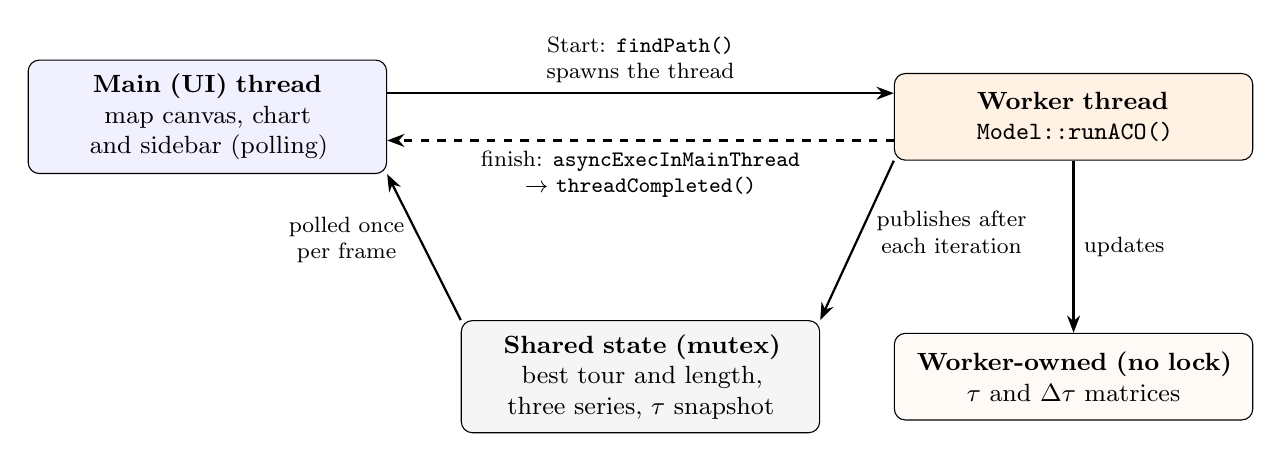
\begin{tikzpicture}[font=\small,
  box/.style={draw,rounded corners,align=center,minimum height=1.1cm,inner sep=5pt,text width=4.2cm},
  lbl/.style={align=center,font=\footnotesize},
  arr/.style={-{Stealth[length=2.2mm]},thick}]
\node[box,fill=blue!6] (ui) at (0,0) {\textbf{Main (UI) thread}\\map canvas, chart\\and sidebar (polling)};
\node[box,fill=orange!10] (wk) at (11,0) {\textbf{Worker thread}\\\texttt{Model::runACO()}};
\node[box,fill=gray!8] (sh) at (5.5,-3.3) {\textbf{Shared state (mutex)}\\best tour and length,\\three series, $\tau$ snapshot};
\node[box,fill=orange!4] (own) at (11,-3.3) {\textbf{Worker-owned (no lock)}\\$\tau$ and $\Delta\tau$ matrices};
\draw[arr] ([yshift=3mm]ui.east) -- node[lbl,above]{Start: \texttt{findPath()}\\spawns the thread} ([yshift=3mm]wk.west);
\draw[arr,dashed] ([yshift=-3mm]wk.west) -- node[lbl,below]{finish: \texttt{asyncExecInMainThread}\\$\rightarrow$ \texttt{threadCompleted()}} ([yshift=-3mm]ui.east);
\draw[arr] (wk.south) -- node[lbl,right]{updates} (own.north);
\draw[arr] (wk.south west) -- node[lbl,right,pos=0.45,xshift=2pt]{publishes after\\each iteration} (sh.north east);
\draw[arr] (sh.north west) -- node[lbl,left,pos=0.55,xshift=-2pt]{polled once\\per frame} (ui.south east);
\end{tikzpicture}
\caption{Division of work between the UI thread and the ACO worker thread.}
\end{figure}

\begin{itemize}
  \item The worker owns $\tau$ and $\Delta\tau$ exclusively and updates them without locking. After each
        complete update it copies $\tau$ into a mutex-guarded snapshot, so the UI can never observe the trail
        mid-evaporation.
  \item The best tour, best length, the three history series, the pheromone snapshot and the view size are
        written only under \code{Model::_mutex}, and the UI thread reads them only under it. (The worker
        also compares against the best length without the lock, which is safe because it is the only
        writer.) The chart's two curves are copied in one lock block, so they always have equal length.
        The sidebar reads the best length under the lock but the iteration counters as separate atomics,
        so for a single frame the counters can lag the best cost by one update.
  \item Counters and flags crossing threads outside the lock (\code{_iteration},
        \code{_bestFoundAtIteration}, \code{_searching}, \code{_stopRequested}, \code{_tourFound},
        \code{_ranToCompletion}, and the live \code{sleepMS} delay) are \code{std::atomic}.
  \item \code{gui::Shape} objects are created only on the main thread. The worker sets
        \code{_tourShapeDirty}; the tour polyline is rebuilt in the next \code{draw()}. The pheromone
        geometry ($O(n^2)$ lines) is rebuilt every 0.15\,s, or immediately after a resize, a new run, new cities
        or a settings change.
  \item Stop only sets \code{_stopRequested}, which the worker checks before each iteration and before each
        ant. Completion is delivered to the main thread with \code{gui::thread::asyncExecInMainThread}, where
        \code{ViewMap::threadCompleted()} joins the thread, stops the timer, stores the run if it completed,
        and refreshes the toolbar. The \code{Model} destructor also requests a stop and joins, and the window
        refuses to close while a run is active.
\end{itemize}

%=====================================================================
\section{GUI Features}
%=====================================================================

The main window (initially $1200\times800$) is a three-row grid: the parameter bar across the top; the map
(15 of 20 columns) with the statistics sidebar beside it (5 columns); and the convergence chart across the
full width, so that successive iterations are as far apart on screen as possible.

\begin{figure}[H]\centering

\includegraphics[width=\linewidth]{main_run.png}
\caption{Main window during a run (16 cities, 20 ants, 40 iterations, $\alpha=1$, $\beta=3$, $\rho=0.5$, random seed,
Threshold pheromone mode), captured at iteration 25. The best tour (888.3\,km, found at iteration 21) is
already 3.7\% shorter than the repetitive nearest-neighbour tour (922.6\,km), which the chart draws as the
horizontal reference line. The thin green lines are the pheromone edges above the threshold.}
\label{fig:main}
\end{figure}

\subsection{Menus and Toolbar}
\begin{itemize}
  \item \textbf{App} menu: Settings, Help, Quit.
  \item \textbf{Animation} menu: Start (checked while running), Reset, New cities, Export run (CSV), Compare
        last 2 runs.
  \item \textbf{Toolbar}: Settings, Start/Stop (icon, label and tooltip switch with the run state), Reset,
        New cities, Export run (CSV), Compare. Toolbar and menu items share action ids and are handled in
        one place (\code{MainWindow::onActionItem}).
\end{itemize}
Reset, New cities, Export and Compare are refused with an explanatory alert while a run is in progress,
because they would either race the worker thread or capture a half-finished run.

\subsection{Parameter Bar}
Number of ants, number of iterations, Alpha, Beta, evaporation rate, a \emph{Speed} slider (delay between
iterations, applied live), a \emph{Path color} picker (the best tour and the best-so-far curve), a
\emph{Start marker} combo box listing the current cities sorted by name, and the \emph{Seed} field
(0 = random).

\subsection{Map Canvas}
\begin{itemize}
  \item \textbf{Pheromone layer} (drawn first): one line per city pair with thickness between 0.5 and 4.0\,px,
        linearly scaled between the smallest and largest current trail value. In \emph{Threshold} mode (the
        default) only edges whose trail exceeds $1.5\times$ the mean over all pairs are drawn, so the layer
        thins out by itself as the colony converges; \emph{All edges} draws every pair.
  \item \textbf{Cities}: grey dots until the first tour exists; cities on the current best tour (after the
        first tour, every city) are drawn in the path colour, with names in dark blue (cyan in dark mode).
        A flag marks the start-marker city.
  \item \textbf{Best tour}: a closed polyline, 5.5\,px, in the path colour.
  \item \textbf{Overlay} (bottom-left): frames per second and elapsed run time.
\end{itemize}
Default colours follow the operating system's theme at start-up (e.g.\ dark red path and blue pheromone
in light mode, orange path and green pheromone in dark mode). With sound enabled, a looping sound plays
while the search runs and a short cheering sound plays when it finishes with a tour.

\subsection{Convergence Chart}
The proposal's primary visualization. It plots, against iteration number $1..N_{\text{iter}}$:
\begin{itemize}
  \item \textbf{Best so far} -- thick line in the path colour, so it reads as the same object as the tour on
        the map;
  \item \textbf{Iteration best} -- thin grey line;
  \item \textbf{Nearest neighbour} -- a horizontal reference line labelled with its length.
\end{itemize}
The vertical range covers both curves \emph{and} the baseline, with 6\% padding. Including the baseline
anchors the scale to a property of the instance: without it, an auto-scaled staircase fills the plot
height whether the run improved by 40\% or by 0.3\%. A status line reports ``Best at iter $a$ (iter $b$/$N$)''
or, after 15 iterations without improvement, ``Converged at iter $a$''. The curves appear once two iterations
have been recorded. Sample $i$ (counting from 0) is plotted at $x=(i+1)/N_{\text{iter}}$, so the ``0'' tick
means ``before the first iteration''.

\subsection{Statistics Sidebar}
\begin{center}
\begin{tabularx}{\linewidth}{@{}l L@{}}
\toprule
\textbf{Row} & \textbf{Meaning} \\
\midrule
Iteration & Current iteration / requested iterations. \\
Best cost & Length of the best tour so far, in km (\texttt{-{}-} before the first tour). \\
Best found at & Iteration that produced the best tour. \\
Nearest neighbour & Repetitive nearest-neighbour tour length for this instance; available before Start. \\
Improvement & Signed percentage by which the best tour is shorter than the baseline. \\
Runtime & Wall-clock time since Start, including the animation delay between iterations. \\
Cities / Ants / Seed & Instance size, colony size, seed (``random'' for 0). \\
Status & Idle; Running; Converged (running, 15 iterations without improvement); Finished (a run ended with a tour). \\
\bottomrule
\end{tabularx}
\end{center}

\subsection{Settings Dialog}
Opened from the toolbar or the App menu. It shows the current language and a language to use after
restart; \emph{Show labels below icons on main toolbar} (applied immediately); \emph{Show town names};
\emph{Play sound while searching}; \emph{Pheromone display} (All edges / Threshold); and \emph{Pheromone
color}. Town names, sound and the pheromone options are populated from the values in force, and the language
from the stored setting, so opening the dialog and pressing OK changes nothing by itself. The toolbar-label
checkbox takes effect as soon as it is clicked. If a different language is selected, the application
offers to restart when the dialog closes.

\begin{figure}[H]\centering

\includegraphics[width=0.6\linewidth]{settings.png}
\caption{The Settings dialog.}
\label{fig:settings}
\end{figure}

\subsection{Compare Dialog}
A read-only dialog built from copies of the two stored run records, so a run started behind it cannot
change its contents. Its contents are described in Section~\ref{sec:compare}.

\begin{figure}[H]\centering

\includegraphics[width=0.8\linewidth]{compare.png}
\caption{Comparison of two completed runs over the same 16 cities, differing only in $\beta$ (5 in the newer
run, 3 in the older). Both reach the same 863.5\,km tour (2.4\% below the nearest-neighbour tour); with
$\beta=5$ the colony finds it two iterations later and its mean iteration best is 3.7\,km higher. Both runs
were made with the speed slider at zero delay, so the runtime of 0.01\,s is essentially the computational cost of
the 40 iterations.}
\label{fig:compare}
\end{figure}

\subsection{Help Dialog}
A static page (App $\rightarrow$ Help) explaining the problem, the search, the map, the chart, the sidebar, the
controls, the settings and reproducibility.

%=====================================================================
\section{Verification: Does the Implementation Match the Proposal?}
%=====================================================================

For this document the complete \code{src/} and \code{res/} trees were cross-checked against the proposal and
against the Ant System as defined by Dorigo and Stützle. The central claim -- every reported tour is the
output of a genuine, live Ant System run, with no precomputed answers and no auxiliary optimizer -- is
confirmed by the control-flow audit below and by an independent numerical re-computation.

\subsection{Control-Flow Audit}
The path from pressing Start to a reported result is a single chain with no bypass:
\begin{verbatim}
MainWindow::onActionItem (Animation/Start)
 -> MainView::startStop
    -> readACOParamsFromUI            (clamp, persist, snapshot parameters)
    -> ViewMap::start
       -> Model::findPath -> reset()  -> std::thread
          -> Model::runACO
             -> buildDistanceMatrix, initPheromone        (dense::DblMatrix)
             -> for iter: for ant:
                  constructTour (roulette, tau^alpha * eta^beta)
                  isHamiltonianTour -> tourLength -> update best (mutex)
             -> evaporatePheromone      (_pheromone *= 1 - rho)
             -> beginPheromoneDeposit   (_deltaPheromone.zeros())
             -> depositPheromone x m    (Q / L_k, symmetric)
             -> applyPheromoneDeposit   (_pheromone += _deltaPheromone)
             -> getL1Norm, publishPheromoneSnapshot, append series (mutex)
          -> asyncExecInMainThread(ViewMap::threadCompleted)
             -> join, stop timer, captureCompletedRun, refresh toolbar
\end{verbatim}
Every best tour shown on the map, plotted on the chart, listed in the sidebar, stored for comparison or
exported passes through \code{constructTour} and \code{isHamiltonianTour} inside this chain.

\subsection{What ``No Cheating'' Means}
\begin{enumerate}
  \item \textbf{No local search.} There is no 2-opt, 3-opt or Or-opt step; tours are exactly as the ants
        built them.
  \item \textbf{No precomputed solutions.} There is no lookup table and no stored tour; each instance is
        drawn at run time.
  \item \textbf{The baseline does not help the colony.} The nearest-neighbour tour is computed separately and
        used only for display and export; $\tau$ is initialized to the constant $\tau_0$, not from the greedy
        tour.
  \item \textbf{No infeasible solutions.} Every tour is verified to be a permutation of all cities before it
        can be reported or reinforced.
  \item \textbf{No elitism or trail limits.} Only the plain Ant System update is applied: no extra deposit
        on the best-so-far tour, no $\tau_{\min}/\tau_{\max}$ bounds.
\end{enumerate}

\subsection{Mathematical Verification}
\begin{enumerate}
  \item \textbf{Transition rule}: the weights are $\tau_{ij}^{\alpha}\eta_{ij}^{\beta}$ with $\eta=1/d$, over unvisited
        cities only, sampled in proportion to weight -- exactly~\eqref{eq:prob}.
  \item \textbf{Update rule}: evaporation of the old trail, accumulation of $Q/L_k$ over all feasible ants
        into $\Delta\tau$, then a single addition -- exactly~\eqref{eq:evap}--\eqref{eq:apply}; deposits are
        symmetric and include the closing edge.
  \item \textbf{Objective}: \code{tourLength} includes the return edge, matching~\eqref{eq:tsp}; the export's
        per-leg column sums to the reported cost up to rounding.
  \item \textbf{Parameters constant}: the ACO fields of \code{Primitive::Options} are written only on the UI
        thread while no run is in progress (at start-up, by \code{readACOParamsFromUI()} on Start, and the seed
        also on New cities) and are only read by the worker.
  \item \textbf{Matrices}: $D$, $\tau$ and $\Delta\tau$ are \code{dense::DblMatrix}; construction reads them through
        manipulators, and evaporation and deposit application are library operators.
\end{enumerate}

\subsection{Independent Numerical Check}\label{sec:numcheck}
To verify correctness against computed output rather than by inspection alone, the instance generator,
the distance computation, the nearest-neighbour baseline and \code{runACO()} were re-implemented
faithfully (same random-number streams, same operations and the same float/double types) in a standalone C++ program and run on the real \code{Bosnia.xml} with the default parameters ($m=20$, 100
iterations, $\alpha=1$, $\beta=3$, $\rho=0.5$, $Q=100$, $\tau_0=1$). For every instance with $n\le20$ the true optimum
was computed with the Held--Karp dynamic program.

\textbf{Distance model.} Over all 4\,755 town pairs more than 20\,km apart, \eqref{eq:dist} differs from
great-circle (haversine) distance by $-1.8\%$ to $+2.0\%$ (mean absolute error 0.4\%, largest absolute
error 4.7\,km). Computing distances through the normalized display coordinates, as the application does,
agrees with~\eqref{eq:dist} to within $2\times10^{-5}$\,km on a test instance (single-precision rounding).

\textbf{Solution quality} (30 instances, seeds 1--30, first city draw):
\begin{center}
\begin{tabular}{@{}lr@{}}
\toprule
\textbf{Measure} & \textbf{Result} \\
\midrule
Instances with exact optimum available ($n\le20$) & 18 \\
ACO best tour equal to the optimum & 10 of 18 \\
Mean gap of ACO to the optimum & 0.68\% \\
Largest gap of ACO to the optimum & 4.12\% \\
Mean gap of repetitive nearest neighbour to the optimum & 7.02\% \\
Largest gap of repetitive nearest neighbour to the optimum & 18.43\% \\
Mean improvement of ACO over nearest neighbour (all 30) & +6.0\% \\
Range of improvement over nearest neighbour & +0.0\% to +16.4\% \\
\bottomrule
\end{tabular}
\end{center}
In no instance was the colony's tour longer than the baseline; in three instances (all with the baseline
already optimal or within 1.7\% of it) the two were equal.

\textbf{Pheromone norm.} Recurrence~\eqref{eq:l1} was checked with random tours on a 20-city instance for 50
iterations: the minimum and maximum column sums of $\tau$ agreed with each other and with the recurrence to
nine decimal places at every iteration.

\begin{figure}[htbp]\centering
\begin{tikzpicture}
\begin{axis}[width=0.95\linewidth,height=6.2cm,xmin=0,xmax=100,ymin=900,ymax=1110,
  xlabel={Iteration},ylabel={Tour length [km]},legend style={font=\small,at={(0.5,-0.22)},anchor=north},legend columns=2,
  tick label style={font=\small},label style={font=\small},grid=major,grid style={gray!20}]
\addplot[gray,thin] table[x index=0,y index=2]{conv.dat};
\addlegendentry{Iteration best}
\addplot[red!60!black,very thick] table[x index=0,y index=1]{conv.dat};
\addlegendentry{Best so far}
\addplot[blue!70!black,dashed,domain=0:100] {1028.8};
\addlegendentry{Repetitive nearest neighbour (1028.8)}
\addplot[black,dotted,thick,domain=0:100] {920.0};
\addlegendentry{Optimum, Held--Karp (920.0)}
\end{axis}
\end{tikzpicture}
\caption{Convergence on one 19-city instance (seed 4) computed by the \emph{reference port}, not a
screenshot of the application. The best tour (920.5\,km, found at iteration 38) is within 0.05\% of the
optimum; the nearest-neighbour tour is 11.8\% above it. The same two curves and baseline are what the
application's convergence chart draws.}
\label{fig:port}
\end{figure}

These figures characterize the algorithm, not a particular run of the application. The port was compiled
with GNU libstdc++; for the reason given in Section~\ref{sec:limits}, the application built with another
standard library will draw different cities and make different ant decisions for the same seed.

\subsection{Known Limitations}\label{sec:limits}
Stated so that no number in the application is read as more than it is:
\begin{itemize}
  \item \textbf{Reproducibility is per toolchain.} \code{std::mt19937} is fully specified, but
        \code{std::shuffle}, \code{std::uniform_int_distribution} and \code{std::uniform_real_distribution} are
        implementation-defined. The same seed reproduces a run on the same platform and standard library
        (for example two Windows builds with MSVC), but not necessarily across MSVC, libc++ (macOS) and
        libstdc++ (Linux). The instance CSV compensates: it contains the full city list and distance matrix,
        so the problem itself can always be reconstructed.
  \item \textbf{Runtime is wall-clock time.} It includes the animation delay between iterations (500\,ms by
        default, so 100 iterations take roughly 50\,s). It measures the presentation, not the computational
        cost; runtime differences in the Compare dialog mostly reflect the speed slider.
  \item \textbf{\code{pheromone_l1} does not measure concentration.} By~\eqref{eq:l1} it is determined by the tour
        lengths alone and is identical for every column; it records total trail mass per city.
  \item \textbf{Stopping mid-iteration} still applies that iteration's pheromone update with the ants that had
        finished, and records the iteration; the worker also finishes the current inter-iteration delay
        (up to 2\,s at the slowest speed) before the run ends. Such a run is marked \code{completed,0} in exports and is not
        stored for comparison.
  \item \textbf{Fixed $\tau_0$.} Dorigo and Stützle suggest $\tau_0=m/C^{\text{nn}}$ for the Ant System; the
        application uses $\tau_0=1$. With $\rho=0.5$ the initial trail falls below 1\% after seven iterations, so
        the choice mainly affects how long the early iterations are dominated by the distance heuristic.
  \item \textbf{Distances are air distances} under a local flat-earth approximation (within $\pm2\%$ of
        great-circle distance), not road distances.
  \item \textbf{``Show town names'' off} shows names only for cities on the best tour. Since every tour contains
        every city, names are hidden only until the first tour exists.
\end{itemize}

\subsection{Conclusion}
The algorithm is a legitimate Ant System. Every reported tour is produced by probabilistic construction
over the natID dense pheromone and distance matrices, validated as a Hamiltonian cycle, and reinforced by
the textbook evaporation-and-deposit rule, with all parameters constant for the run. There is no local
search, no precomputed solution, and no use of the greedy baseline inside the search. In the independent re-computation with
the default parameters, the same algorithm reached the exact optimum in 10 of the 18 instances that could be
solved exactly and stayed within 0.7\% of it on average.

%=====================================================================
\section{Conclusions}
%=====================================================================

\subsection{What the Project Demonstrates}
ACO TSP Solver shows end to end how a population-based metaheuristic solves an NP-hard combinatorial
problem with nothing more than two matrices and one feedback rule: ants read $\tau$ and $D$ to build tours,
the tours write back into $\tau$ in proportion to their quality, and evaporation keeps the colony from
locking onto its first guesses. The live map makes that feedback visible -- the pheromone layer starts
uniform and collapses onto a handful of edges -- while the convergence chart and the nearest-neighbour
baseline turn ``it seems to work'' into a measurable claim.

\subsection{Problems It Solves}
\begin{itemize}
  \item Provides a concrete, inspectable answer to ``how does Ant Colony Optimization actually work'', down
        to individual matrix entries and random draws.
  \item Gives a sandbox for studying the effect of $\alpha$, $\beta$, $\rho$, colony size and run length on real
        geographic instances, with side-by-side comparison of two runs.
  \item Produces analysis-ready data: the convergence series for plotting, and a self-contained instance
        file from which any reported tour length can be checked with a spreadsheet formula.
  \item Anchors every result to an external reference (a strong greedy tour), so a run that fails to beat it
        is reported as such.
\end{itemize}

\subsection{Lessons Learned}
\begin{itemize}
  \item \textbf{A best-so-far curve alone proves little.} It is monotone by construction and fills any
        auto-scaled chart. The per-iteration best and a fixed baseline are what make convergence observable.
  \item \textbf{A solver must check its own constraints.} An infeasible tour is cheaper than a feasible one, so a
        construction bug would look like a spectacular result rather than a failure.
  \item \textbf{Instrumentation must be checked against the mathematics.} The pheromone $L_1$ norm looked like a
        convergence signal, but the Hamiltonian structure of every tour makes all column sums equal, so it
        cannot measure concentration.
  \item \textbf{Threading discipline is part of correctness.} A worker-owned matrix plus published snapshots,
        atomics for cross-thread flags, and main-thread-only graphics objects kept a live visualization from
        ever reading half-updated state.
  \item \textbf{Reproducibility needs more than a seed.} The city-draw index is required to identify an instance,
        and standard-library distributions differ between platforms.
\end{itemize}

\subsection{Possible Future Work}
\begin{itemize}
  \item \textbf{Stronger ACO variants}: Ant Colony System (pseudo-random proportional rule, local update) and
        MAX--MIN Ant System (trail limits, best-ant deposit), selectable at run time for comparison.
  \item \textbf{Local search}: a 2-opt step on each constructed tour, which typically closes the remaining gap
        to the optimum.
  \item \textbf{A real concentration measure}: for example the mean entropy of the rows of the normalized
        transition probabilities, or the share of total trail on the current best tour's edges, to replace
        \code{pheromone_l1} in the export.
  \item \textbf{Platform-independent randomness}: hand-written uniform sampling on top of \code{std::mt19937}, so
        a seed reproduces a run identically on every platform.
  \item \textbf{Larger and external instances}: loading TSPLIB files and reporting the gap to their known
        optima.
\end{itemize}

\section*{References}
\addcontentsline{toc}{section}{References}
\begin{enumerate}[label={[\arabic*]}]
  \item M. Dorigo, T. Stützle, \emph{Ant Colony Optimization}, MIT Press, Cambridge, MA, 2004.
  \item A. Memišević, \emph{Ant Colony Optimization for the Traveling Salesman Problem} -- project proposal,
        ETF Sarajevo (\code{Documents/NO_project_proposal_ArminMemisevic.pdf}).
  \item I. Džafić, \emph{natID} framework and the \code{B_S03_Maps} example,
        \url{https://github.com/idzafic/natID}.
  \item Project repository: \url{https://github.com/arminn2206/ProjNO_TSPACO_Memisevic}.
\end{enumerate}

\end{document}
